% =========================================================
% Section: Process API
% =========================================================

\section{Process API}

% ---------------------------------------------------------
\begin{frame}{Process Creation and Control}

\begin{block}{Key Question}
What interfaces should the operating system provide for
\textbf{process creation and control}?
\end{block}

\begin{itemize}
    \item UNIX provides a distinctive process creation API.
    \item Three fundamental system calls:
    \begin{itemize}
        \item \texttt{fork()} -- create a new process;
        \item \texttt{exec()} -- execute a different program;
        \item \texttt{wait()} -- wait for a child process to finish.
    \end{itemize}
\end{itemize}

\end{frame}

% ---------------------------------------------------------
\begin{frame}{The \texttt{fork()} System Call}

\begin{columns}[T]

\begin{column}{0.47\textwidth}
\begin{itemize}
    \item \texttt{fork()} creates a new process.
    \item The original process is the \textbf{parent}.
    \item The newly created process is the \textbf{child}.
    \item The child is an almost exact copy of the parent.
    \item Both continue execution after \texttt{fork()}.
\end{itemize}

\begin{block}{Return Value}
\begin{itemize}
    \item Parent: child PID.
    \item Child: \texttt{0}.
    \item Failure: negative value.
\end{itemize}
\end{block}
\end{column}

\begin{column}{0.50\textwidth}
\begin{figure}
    \centering
    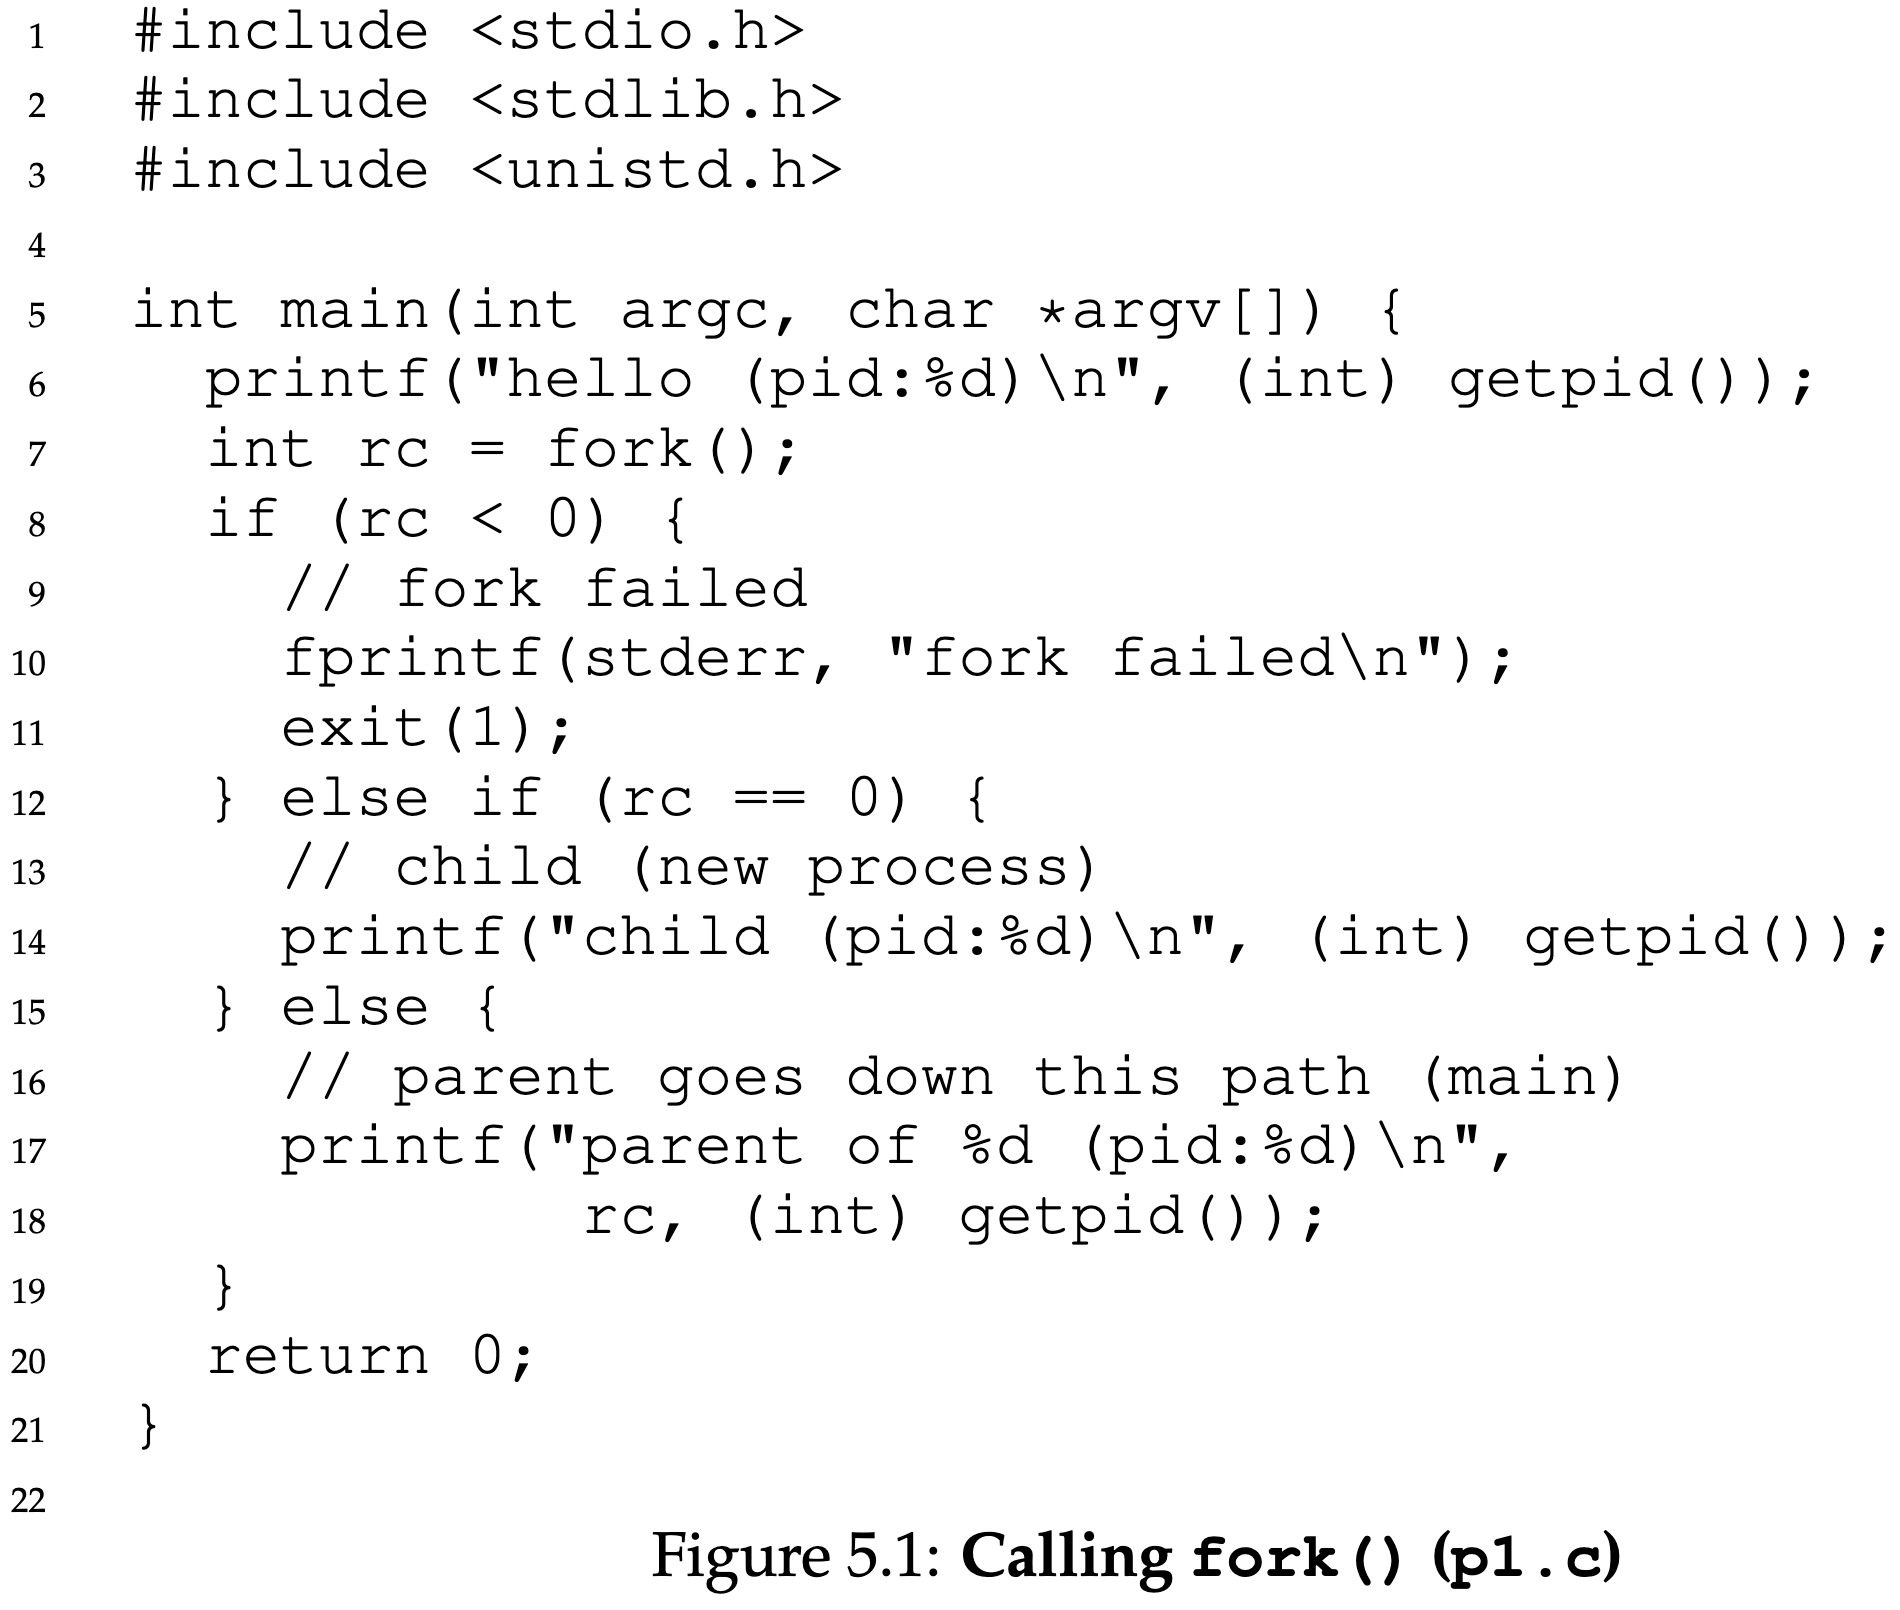
\includegraphics[width=1.1\linewidth]{figs/chapter-5/figure-5.1.png}
    \caption*{Source: chapter page 2.}
    \label{fig:figure-5.1}
\end{figure}
\end{column}

\end{columns}

\end{frame}

% ---------------------------------------------------------
\begin{frame}{Parent and Child Execution}

\begin{itemize}
    \item Each process has its own:
    \begin{itemize}
        \item address space;
        \item registers;
        \item program counter.
    \end{itemize}

    \item Parent and child may execute in different orders.
    \item The scheduler determines which process runs first.
    \item Execution after \texttt{fork()} is therefore
          \textbf{non-deterministic}.
\end{itemize}

\vspace{0.3cm}

\begin{block}{Process Identifier}
Each process is identified by a unique \textbf{PID}
(Process Identifier).
\end{block}

\end{frame}

% ---------------------------------------------------------
\begin{frame}{The \texttt{wait()} System Call}

\begin{columns}[T]

\begin{column}{0.45\textwidth}

\begin{itemize}
    \item A parent may need to wait for a child to finish.
    \item \texttt{wait()} blocks the parent.
    \item The parent becomes runnable again after the child terminates.
    \item This can make execution order predictable.
\end{itemize}

\vspace{0.2cm}

\begin{block}{Execution Order}
With \texttt{wait()}, the child completes before the parent continues
past the system call.
\end{block}

\end{column}

\begin{column}{0.52\textwidth}
\begin{figure}
    \centering
    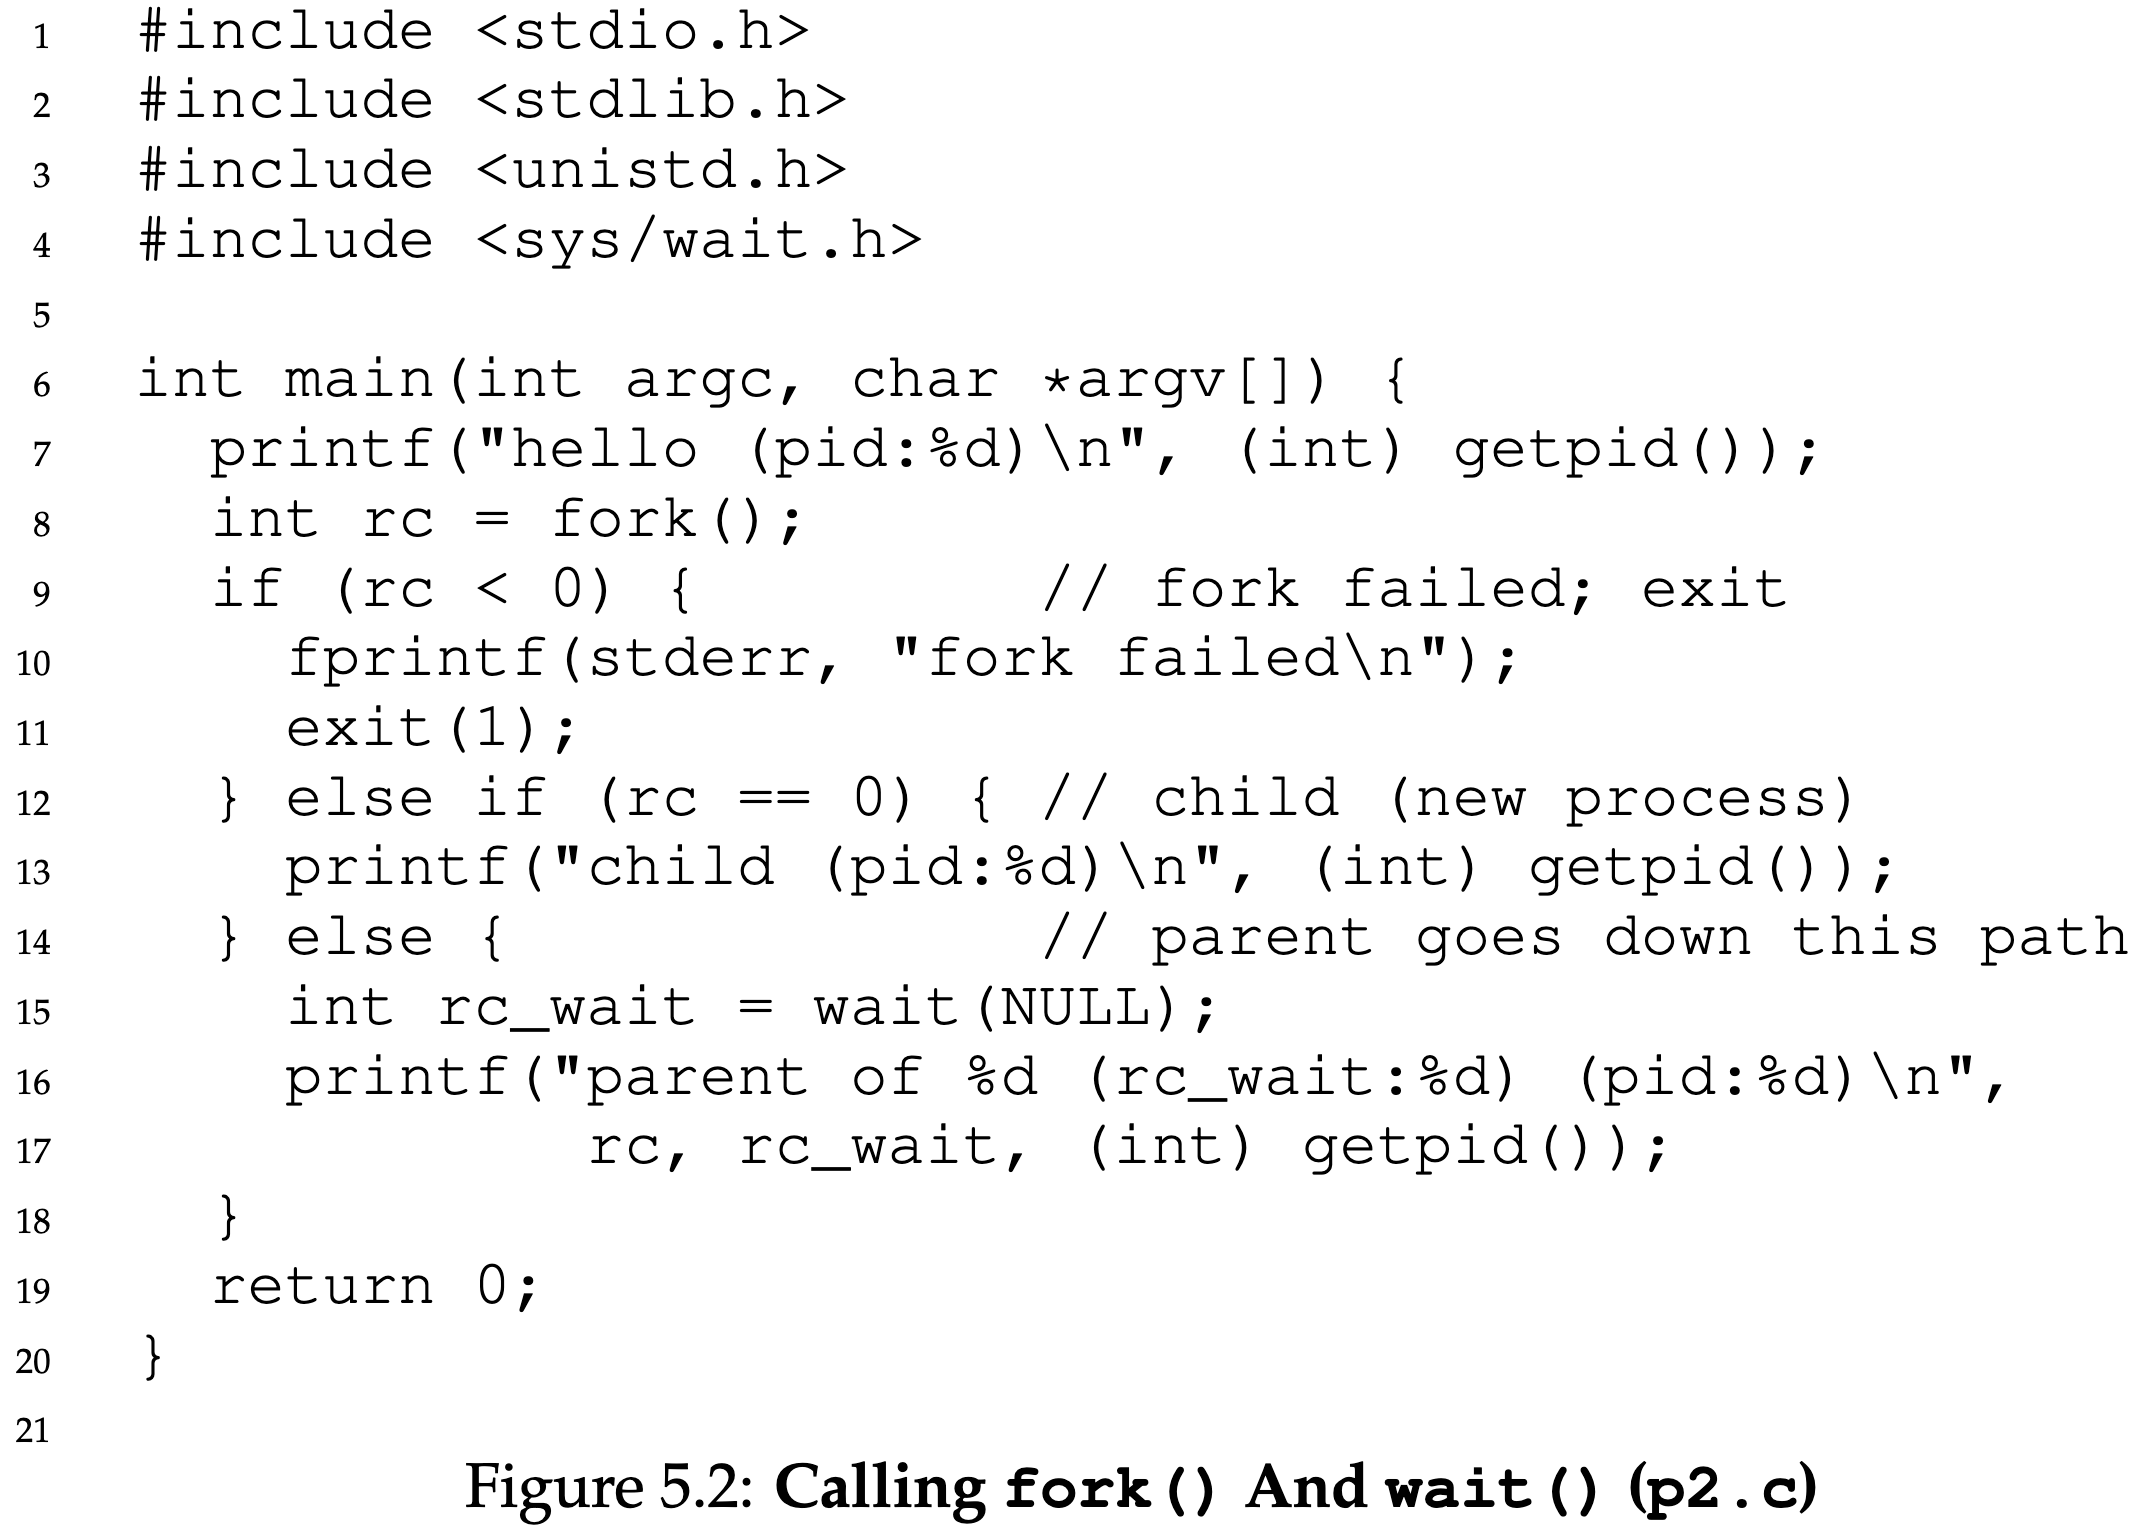
\includegraphics[width=1.1\linewidth]{figs/chapter-5/figure-5.2.png}
    \caption*{Source: chapter page 3.}
    \label{fig:figure-5.2}
\end{figure}
\end{column}

\end{columns}

\end{frame}

% ---------------------------------------------------------
\begin{frame}{The \texttt{exec()} System Call}

\begin{columns}[T]

\begin{column}{0.44\textwidth}

\begin{itemize}
    \item \texttt{exec()} runs a different program.
    \item It replaces the current process image.
    \item Code and static data are replaced.
    \item Heap and stack are re-initialized.
    \item It does \textbf{not} create a new process.
    \item A successful \texttt{exec()} does not return.
\end{itemize}

\end{column}

\begin{column}{0.53\textwidth}
\begin{figure}
    \centering
    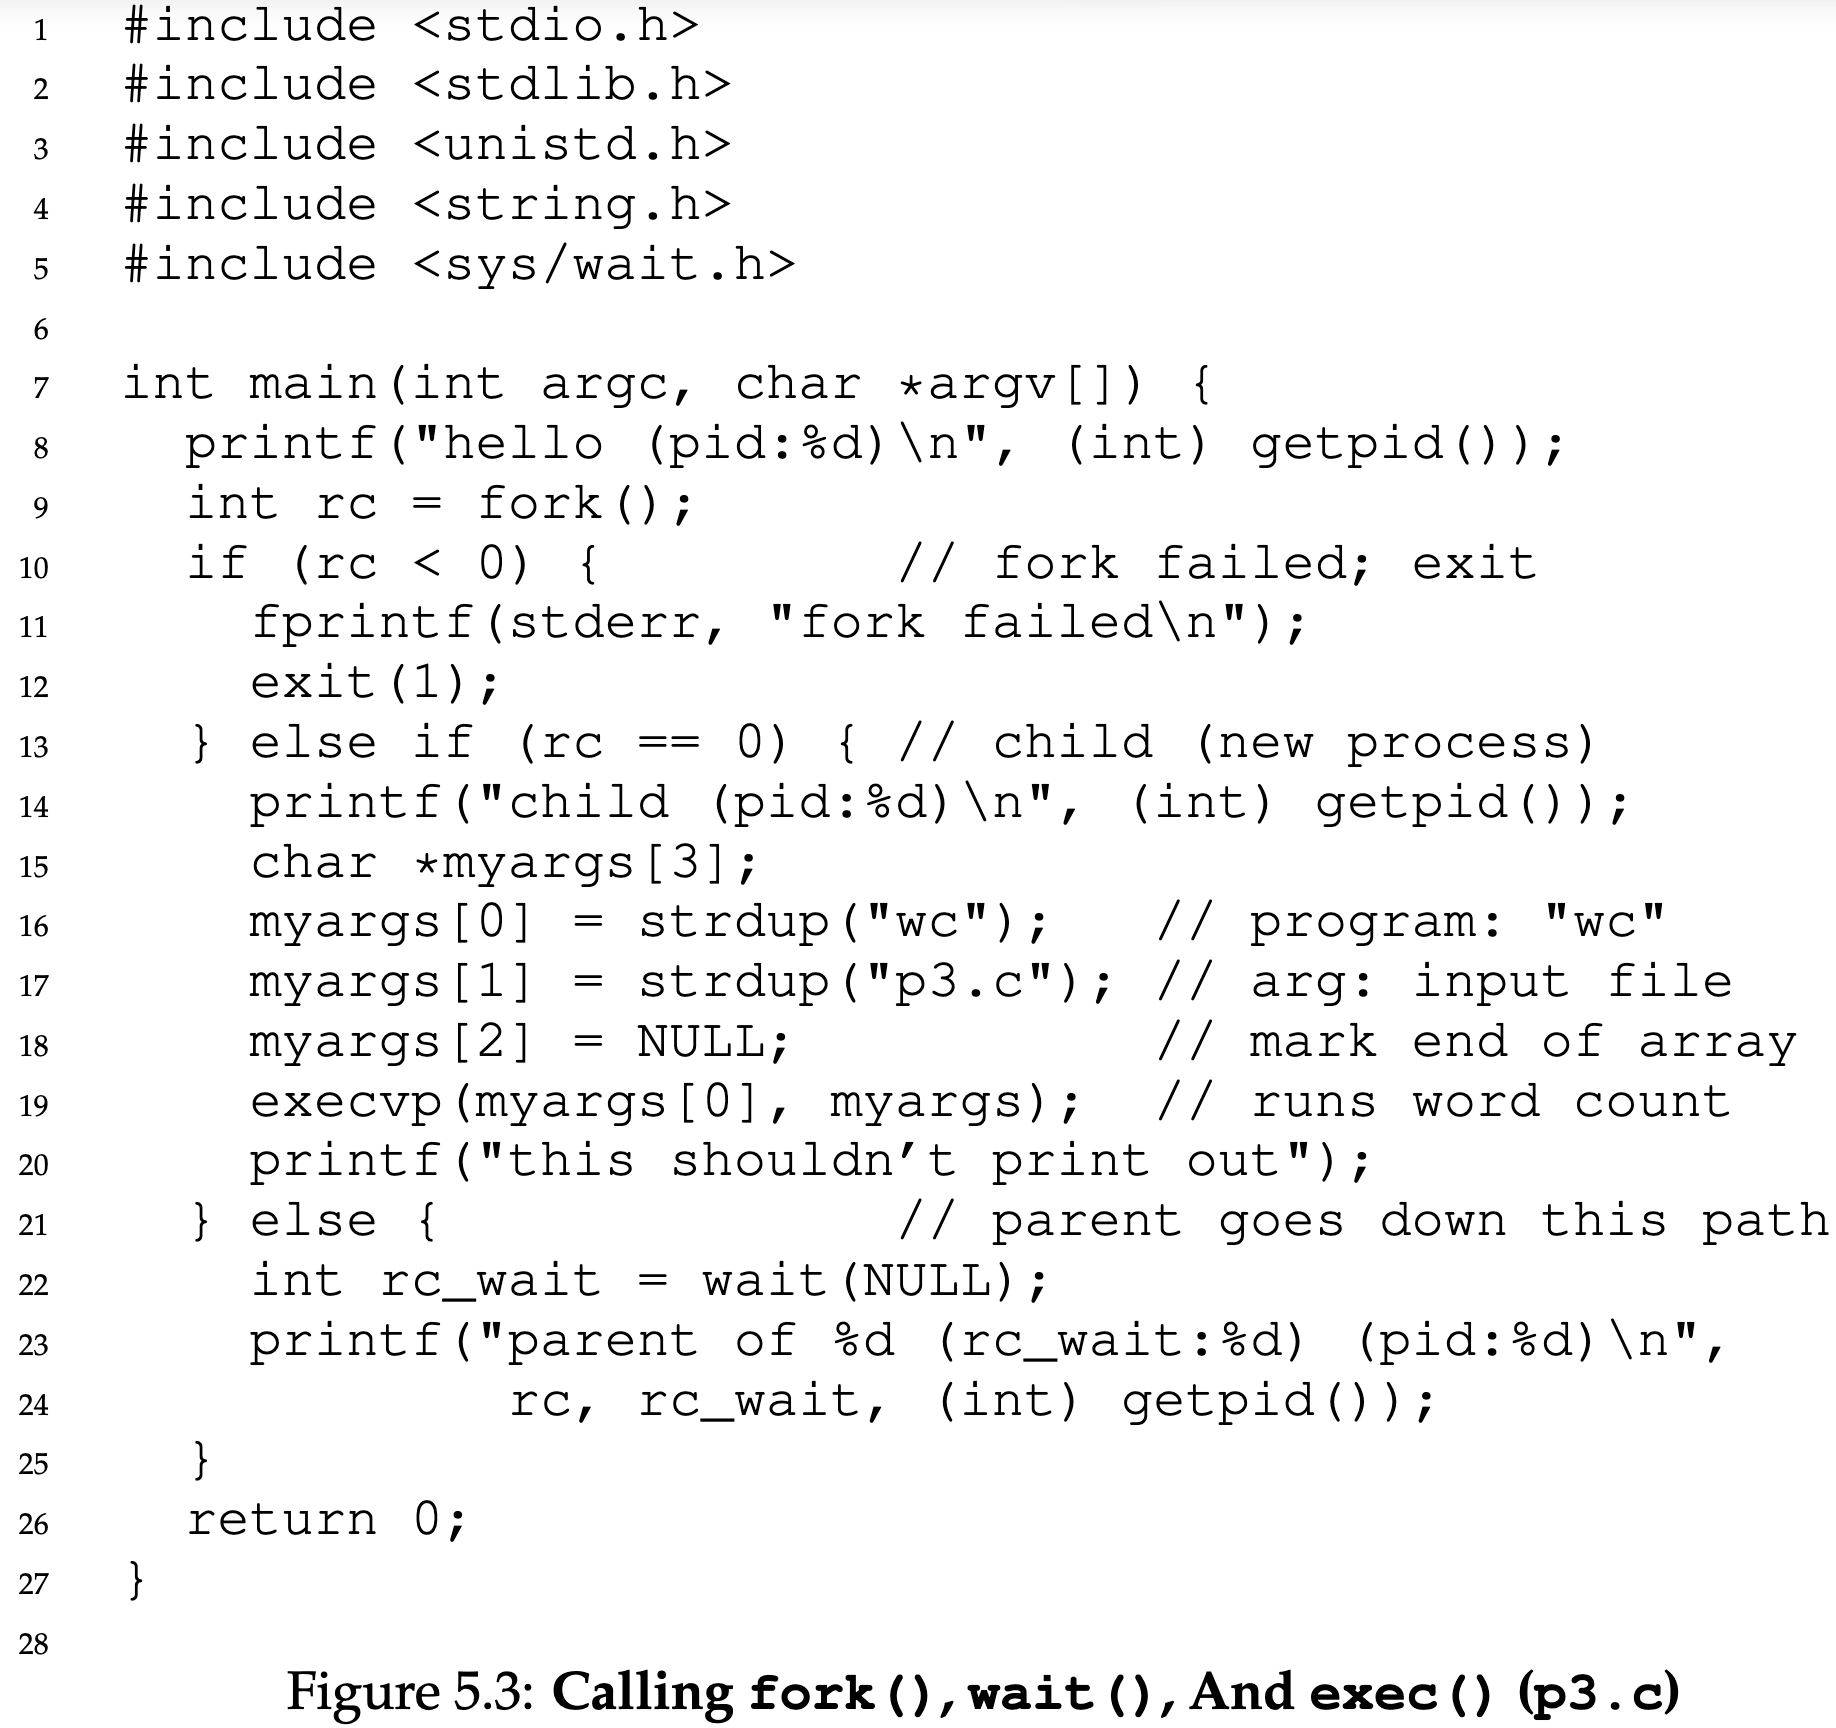
\includegraphics[width=1.1\linewidth]{figs/chapter-5/figure-5.3.png}
    \caption*{Source: chapter page 5.}
    \label{fig:figure-5.3}
\end{figure}
\end{column}

\end{columns}

\end{frame}

% ---------------------------------------------------------
\begin{frame}{Why Separate \texttt{fork()} and \texttt{exec()}?}

\begin{itemize}
    \item The separation is essential to the design of the UNIX shell.
    \item A shell typically:
    \begin{enumerate}
        \item reads a command;
        \item calls \texttt{fork()};
        \item modifies the child's environment if necessary;
        \item calls \texttt{exec()};
        \item waits for completion with \texttt{wait()}.
    \end{enumerate}
\end{itemize}

\vspace{0.3cm}

\begin{block}{Key Advantage}
The shell can perform operations \textbf{between}
\texttt{fork()} and \texttt{exec()}.
\end{block}

\end{frame}

% ---------------------------------------------------------
\begin{frame}[fragile]{I/O Redirection}

\begin{columns}[T]

\begin{column}{0.42\textwidth}

Example:

\begin{verbatim}
wc p3.c > newfile.txt
\end{verbatim}

\begin{itemize}
    \item The shell creates a child with \texttt{fork()}.
    \item The child closes standard output.
    \item It opens the destination file.
    \item The file becomes the new standard output.
    \item File descriptors remain open across \texttt{exec()}.
\end{itemize}

\end{column}

\begin{column}{0.55\textwidth}
\begin{figure}
    \centering
    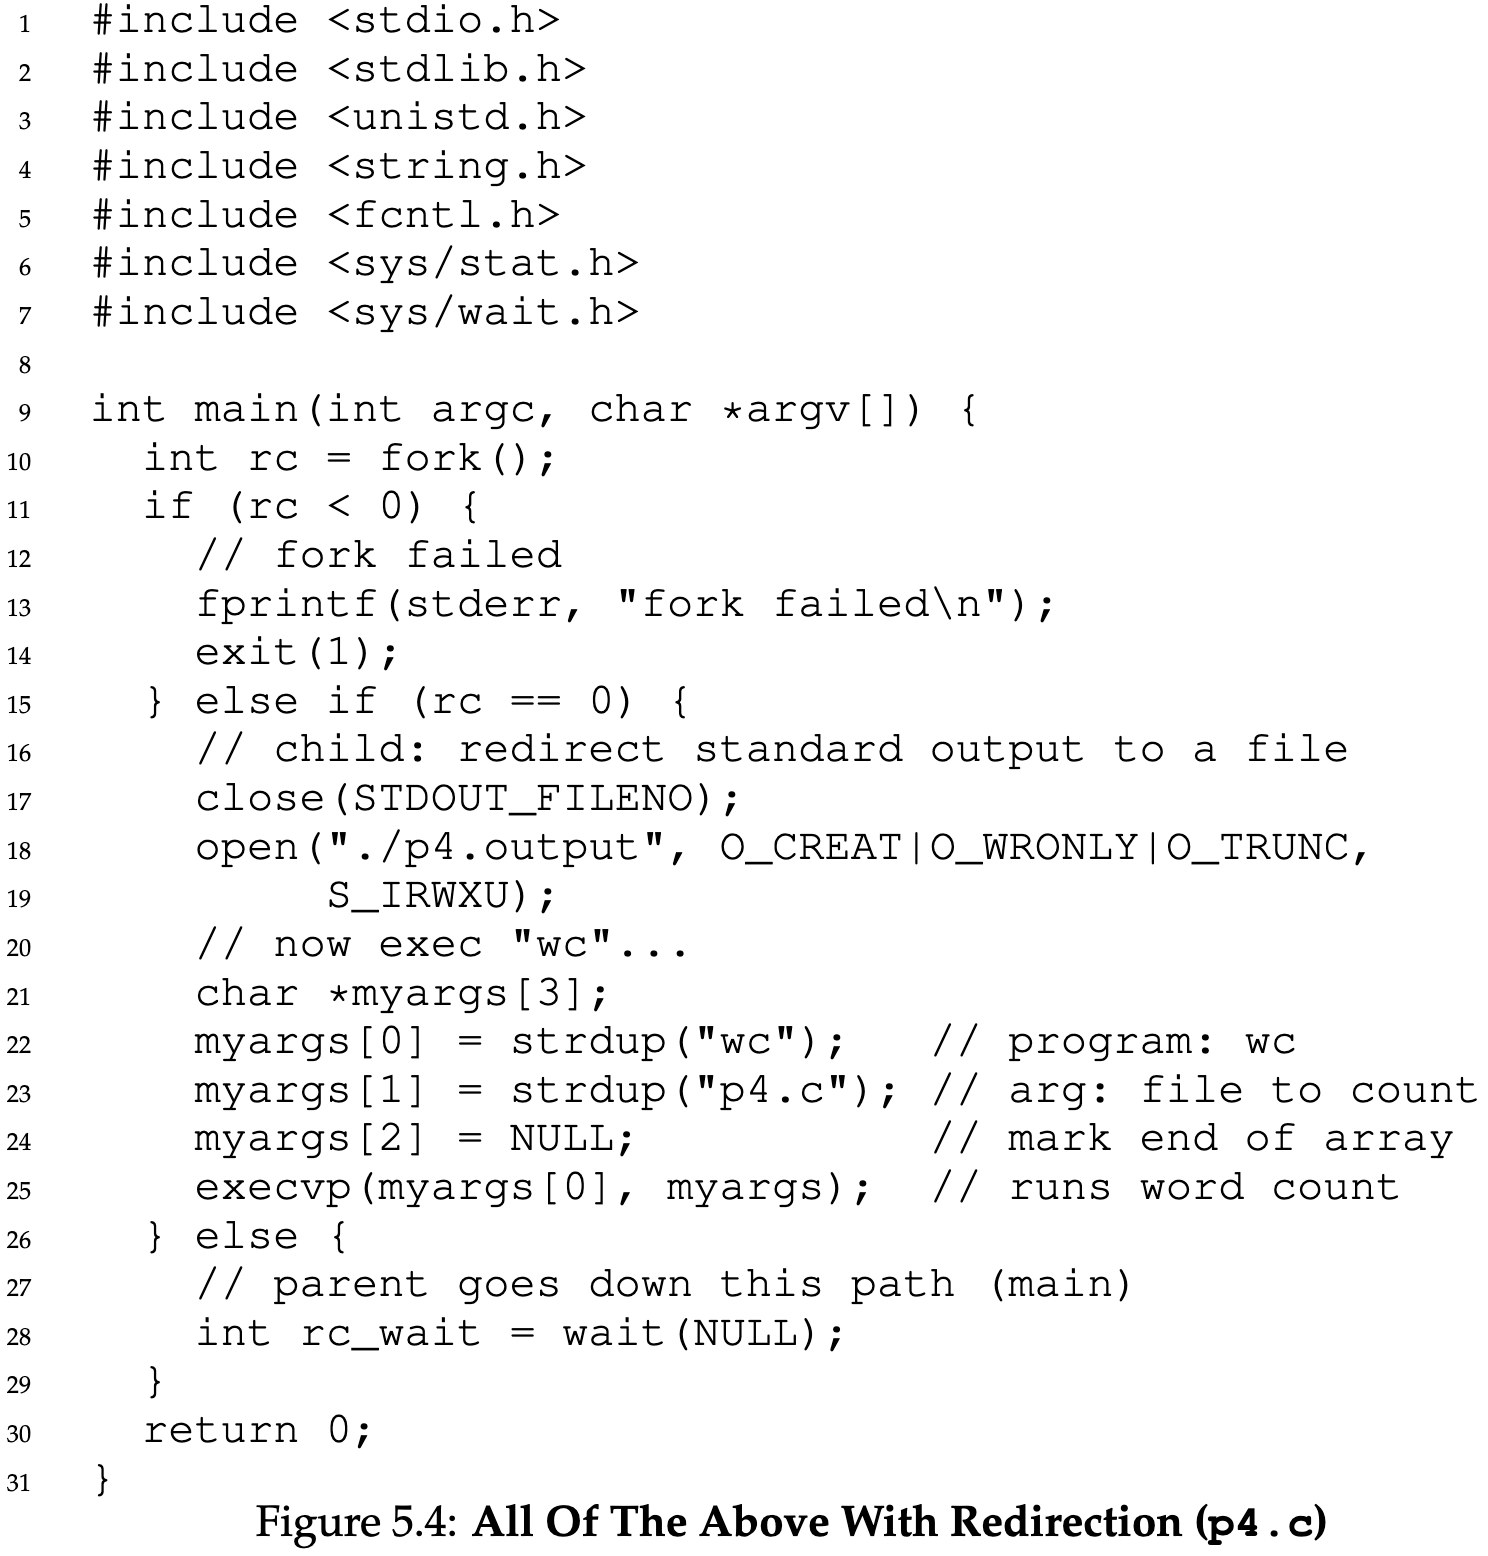
\includegraphics[width=1.1\linewidth]{figs/chapter-5/figure-5.4.png}
    \caption*{Source: chapter page 8.}
    \label{fig:figure-5.4}
\end{figure}
\end{column}

\end{columns}

\end{frame}

% ---------------------------------------------------------
\begin{frame}[fragile]{Pipes}

\begin{itemize}
    \item UNIX pipes use the \texttt{pipe()} system call.
    \item The output of one process is connected to an
          in-kernel pipe.
    \item The input of another process is connected to the same pipe.
    \item This allows commands to be combined into processing chains.
\end{itemize}

\vspace{0.3cm}

\begin{exampleblock}{Example}
\begin{verbatim}
grep -o foo file | wc -l
\end{verbatim}
\end{exampleblock}

The output of \texttt{grep} becomes the input of \texttt{wc}.

\end{frame}

% ---------------------------------------------------------
\begin{frame}{Process Control and Signals}

\begin{itemize}
    \item UNIX provides additional interfaces for process control.
    \item \texttt{kill()} sends signals to processes.
    \item Signals can stop, continue, interrupt, or terminate processes.
\end{itemize}

\vspace{0.2cm}

\begin{block}{Common Shell Shortcuts}
\begin{itemize}
    \item \texttt{Ctrl+C} $\rightarrow$ \texttt{SIGINT}
    \item \texttt{Ctrl+Z} $\rightarrow$ \texttt{SIGTSTP}
    \item \texttt{fg} can resume a stopped job.
\end{itemize}
\end{block}

\begin{itemize}
    \item Processes can use \texttt{signal()} to react to signals.
\end{itemize}

\end{frame}

% ---------------------------------------------------------
\begin{frame}{Users and Process Control}

\begin{itemize}
    \item UNIX systems support multiple users.
    \item Users generally control only their own processes.
    \item The operating system protects processes belonging to
          different users.
    \item The \textbf{superuser} (\texttt{root}) has broader privileges.
    \item Root can control processes belonging to other users.
\end{itemize}

\vspace{0.3cm}

\begin{alertblock}{Superuser}
Administrative privileges should be used carefully because they provide
extensive control over the system.
\end{alertblock}

\end{frame}

% ---------------------------------------------------------
\begin{frame}{Useful Process Tools}

\begin{itemize}
    \item \texttt{ps} -- displays running processes.
    \item \texttt{top} -- displays processes and resource usage.
    \item \texttt{kill} -- sends signals to processes.
    \item \texttt{killall} -- another interface for sending signals.
\end{itemize}

\vspace{0.3cm}

\begin{block}{Good Practice}
Use UNIX \texttt{man} pages to study system calls,
return values, options, and error conditions.
\end{block}

\end{frame}

% ---------------------------------------------------------
\begin{frame}{Process API: Summary}

\begin{itemize}
    \item \texttt{fork()} creates a new child process.
    \item \texttt{wait()} allows a parent to wait for a child.
    \item \texttt{exec()} replaces the current program with another.
    \item UNIX shells combine these mechanisms to execute commands.
    \item The separation of \texttt{fork()} and \texttt{exec()}
          enables redirection and pipes.
    \item Signals provide mechanisms for process control.
    \item Users and permissions determine which processes can be controlled.
\end{itemize}

\end{frame}